\documentclass[12pt,a4paper]{report}
\usepackage{siunitx}
\usepackage{amsmath}
\usepackage{amsfonts}
\usepackage{amssymb}
\usepackage[bottom]{footmisc}
\usepackage{verbatim}
\usepackage{graphicx}
\usepackage[utf8]{inputenc}
\usepackage[english]{babel}
\usepackage[left=3cm,right=3cm,top=3cm,bottom=3cm]{geometry}
%\usepackage[small,compact]{titlesec}
\usepackage{setspace}
\usepackage{hyperref,cleveref}
\usepackage{cite}
\usepackage{color}
%\usepackage{tikz}
\usepackage{caption}
\usepackage{subcaption}
\usepackage{siunitx}
\usepackage{url}
\usepackage[round]{natbib}
\usepackage{gensymb}
\usepackage{geometry}
\usepackage{upgreek}

% Define stuff here
\def\albatros{ALBATROS}
\def\prizm{PRI$^{\rm Z}$M}
\newcommand{\attention}[1]{\textcolor{red}{\bf {#1}}}

\newcommand{\ieee}{Institute of Electrical and Electronics Engineers}
\newcommand{\aap}{Astronomy and Astrophysics}
\newcommand{\aaps}{Astronomy and Astrophysics Supplements}
\newcommand{\aj}{Astronomical Journal}
\newcommand{\apj}{Astrophysical Journal}
\newcommand{\jgr}{Journal of Geophysical Research}
\newcommand{\mnras}{Monthly Notices of the Royal Astronomical Society}
\newcommand{\nar}{New Astronomy Reviews}
\newcommand{\pasa}{Publications of the Astronomical Society of Australia}
\newcommand{\pasp}{Proceedings of the Astronomical Society of the Pacific}
\newcommand{\prd}{Physical Review D}
\newcommand{\prl}{Physical Review Letters}
\newcommand{\araa}{Annual Review of Astronomy and Astrophysics}
\newcommand{\apjl}{The Astrophysical Journal Letters }
\newcommand{\apjs}{The Astrophysical Journal Supplement Series}
\newcommand{\physrep}{Physical Reports}
\newcommand{\jrasc}{Journal of the Royal Astronomical Society of Canada}


\begin{document}
	\begin{titlepage}
		
		\newcommand{\HRule}{\rule{\linewidth}{0.5mm}} % Defines a new command for the horizontal lines, change thickness here
		
		\begin{center}
		\begin{figure}[ht]
			\centering
				
\includegraphics[width=0.5\textwidth]{Figures/UKZNLOGO.png}\\[1cm]
		\end{figure}
		
		\LARGE {\textbf {Low-Frequency Observations of the Radio\\[0.3cm Sky from Marion Island]}}\\[1cm]
	    {By}\\[0.5cm]
		\textbf {\Large {Tankiso H. Moso}}\\[0.5cm]
		{\small Submitted in the School of Mathematics, Statistics and Computer Sciences\\in  fulfilment of the academic requirements for the\\Master of Science Degree in Applied Mathematics\\at the\\University of Kwa-Zulu Natal}\\[1cm]
		
		{\large Supervisor: Prof. H. C. Chiang}\\[0.1cm]
		{\large Co-Supervisor: Prof. K. Moodley}\\[3cm]
		
		{\large \today}\\[0cm] % Date, change the \today to a set date if you want to be precise
		\end{center}	
	\end{titlepage}

\pagenumbering{roman}

\addcontentsline{toc}{section}{Declaration}
\section*{Declaration - Plagiarism}

I, Tankiso Moso, declare that

\begin{enumerate}
	\item The research reported in this thesis, except where otherwise indicated, is my original research.
	\item This thesis has not been submitted for any degree or examination at any other university.
	\item This thesis does not contain other persons’ data, pictures, graphs or other information, unless specifically acknowledged as being sourced from other persons.
	\item This thesis does not contain other persons' writing, unless specifically acknowledged as being sourced from other researchers.  Where other written sources have been quoted, then:
\begin{enumerate}
	\item Their words have been re-written but the general information attributed to them has been referenced.
	\item Where their exact words have been used, then their writing has been placed in italics and inside quotation marks, and referenced.
\end{enumerate}
		
	\item This thesis does not contain text, graphics or tables copied and pasted from the internet, unless specifically acknowledged, and the source being detailed in the thesis and in the References section.
\end{enumerate}
\vspace{0.5cm}
	
\begin{table}[h]
\begin{tabular}{c}
\hline
Tankiso H. Moso\\
\end{tabular}
\end{table}	
{\large \today}\\ % Date, change the \today to a set date if you want to be precise %Change the date to your date of submission


\newpage
\section*{Abstract}
Measurements of the radio sky at frequencies below $\sim$100 MHz have the potential to unlock a new observational window into the universe’s history. These observations allow us to probe even earlier epochs of the universe’s history and lay the groundwork for eventually
exploring the cosmic “dark ages”. There is minimal knowledge about the radio sky below 30 MHz. The lowest measured frequency of the radio sky was dated from the 1960s when Grote Reber mapped a portion of the sky at $ \sim $ 2 MHz using a 192-element dipole array with $\sim$5 \degree
resolution. This brief glimpse of low-frequency Galactic emission was made possible partly by an unusually deep solar minimum.\\

The Array of Long Baseline Antennas for Taking Radio Observations from the Sub-Antarctic (ALBATROS) will be a new interferometric array that aims to provide improved images of the radio sky at low frequencies. The array will consist of approximately 10 antenna stations operating at 1.2 MHz to 125 MHz, with a maximum baseline length of $\sim$ 20 km. Potential ALBATROS station locations form a ring-like pattern that is appropriate for imaging, and produce a Full Width at Half Maximum (FWHM) synthesized beam of \SI{7}{\arcminute} at 5 MHz. This
beam represents a notable advance over measurements to date. The antenna stations will operate autonomously and record baseband data in a selected $ \sim $ 10 MHz frequency window. The data from all stations will be post-processed and interferometrically combined
offline. \\

Preliminary observations from the pathfinder installed in April 2018 show discernible interferometric fringes from the sky visible down to $\sim$ 10 MHz without any data processing or cuts. The first fully autonomous antenna station was deployed in April 2019, configured to record baseband data, and with power supplied by solar panels. 


\newpage
\section*{Acknowledgements}

\newpage
\renewcommand\contentsname{Table of Contents} %This changes the original latex contents name to 'Table of Contents'
\tableofcontents\newpage %This adds the table of contents to your thesis.

	
\pagenumbering{arabic}	


\chapter{Introduction}

	Our Universe’s origin has always been a mystery until the last few decades when humankind started looking for answers to the unanswered questions about the evolution of the Universe. The process of finding solutions to problems that arose built up to a field of study called cosmology. This field has drastically impacted our knowledge of the universe evolution~\citep{book:909085}.
		
	The primordial humankind assumed that the Sun, the moon, and other planets orbited the Earth until Nicolaus Copernicus and other astronomers replaced the geocentric model with the heliocentric model~\citep{2015arXiv150201967R}.
		
	The celestial mechanics area of study came into existence after Isaac Newton made discoveries that the elliptic planet motion, among other things, can be explained by gravitational force attraction~\citep{2015arXiv150201967R}. He also reasoned that the Kepler ellipse is only an approximation of the true nature of planetary motion (interaction between planets)~\citep{2015arXiv150201967R,2015arXiv150704654N}. In the modern study of the Universe, Albert Einstein has been a significant influence on the theory of general relativity. This theory presents the mathematical framework required to explain the evolution of the universe~\citep{2018EPJH...43...73O}.
		
	As a result of all these findings, Georges Lemaitre proposed the Big Bang theory, which is the contemporary model that provides a complete explanation of the Universe expansion~\citep{2020AntAs..14....2M}. This theory was established from Hubble’s law and subsequently by Arno Penzias and Robert Wilson in 1964 from discovering the cosmic microwave background (CMB)~\citep{2018EPJH...43...73O,2003RvMP...75..559P,1929PNAS...15..168H}.
		
	Later on, there were obvious unforeseen observations of the acceleration of the Universe. The Supernova Cosmology Project and the High-Z Supernovae Search Team in 1998 uncovered the acceleration of the Universe. They used type Ia supernovae to determine the acceleration of the Universe~\citep{1998AJ....116.1009R, 1999ApJ...517..565P}. The Universes expansion acceleration is described by the dark energy that accounts for approximately 74 percent of the Universe’s energy density. Today, any discoveries of dark energy are still as disconcerting in the study of astrophysics and particle physics~\citep{2008ARA&A..46..385F, 2015Sci...349..849H}.\\
		
	\section{History of the Universe}
	

	\autoref{Fig:timeline} shows the cosmic history of the Universe, where the earliest era was the Planck era. It is from zero to \SI{e-43}{s} from the birth of the Universe. Before the \SI{e-43}{s} era, it is unknown to physicists what happened, the only progress made was to build up from the \SI{e-43}{s} from the birth of the Universe. To understand what happened before \SI{e-43}{s}, one needs to know the quantum theory of gravity~\citep{2015Sci...349..849H}. What was deduced from the Planck era was the rapid exponential expansion of the Universe, which is governed by the Epoch of Inflation. It is \SI{e-34}{s} from the birth of the Universe~\citep{Planck}.
	
	\begin{figure}[htb!]
		\begin{center}
			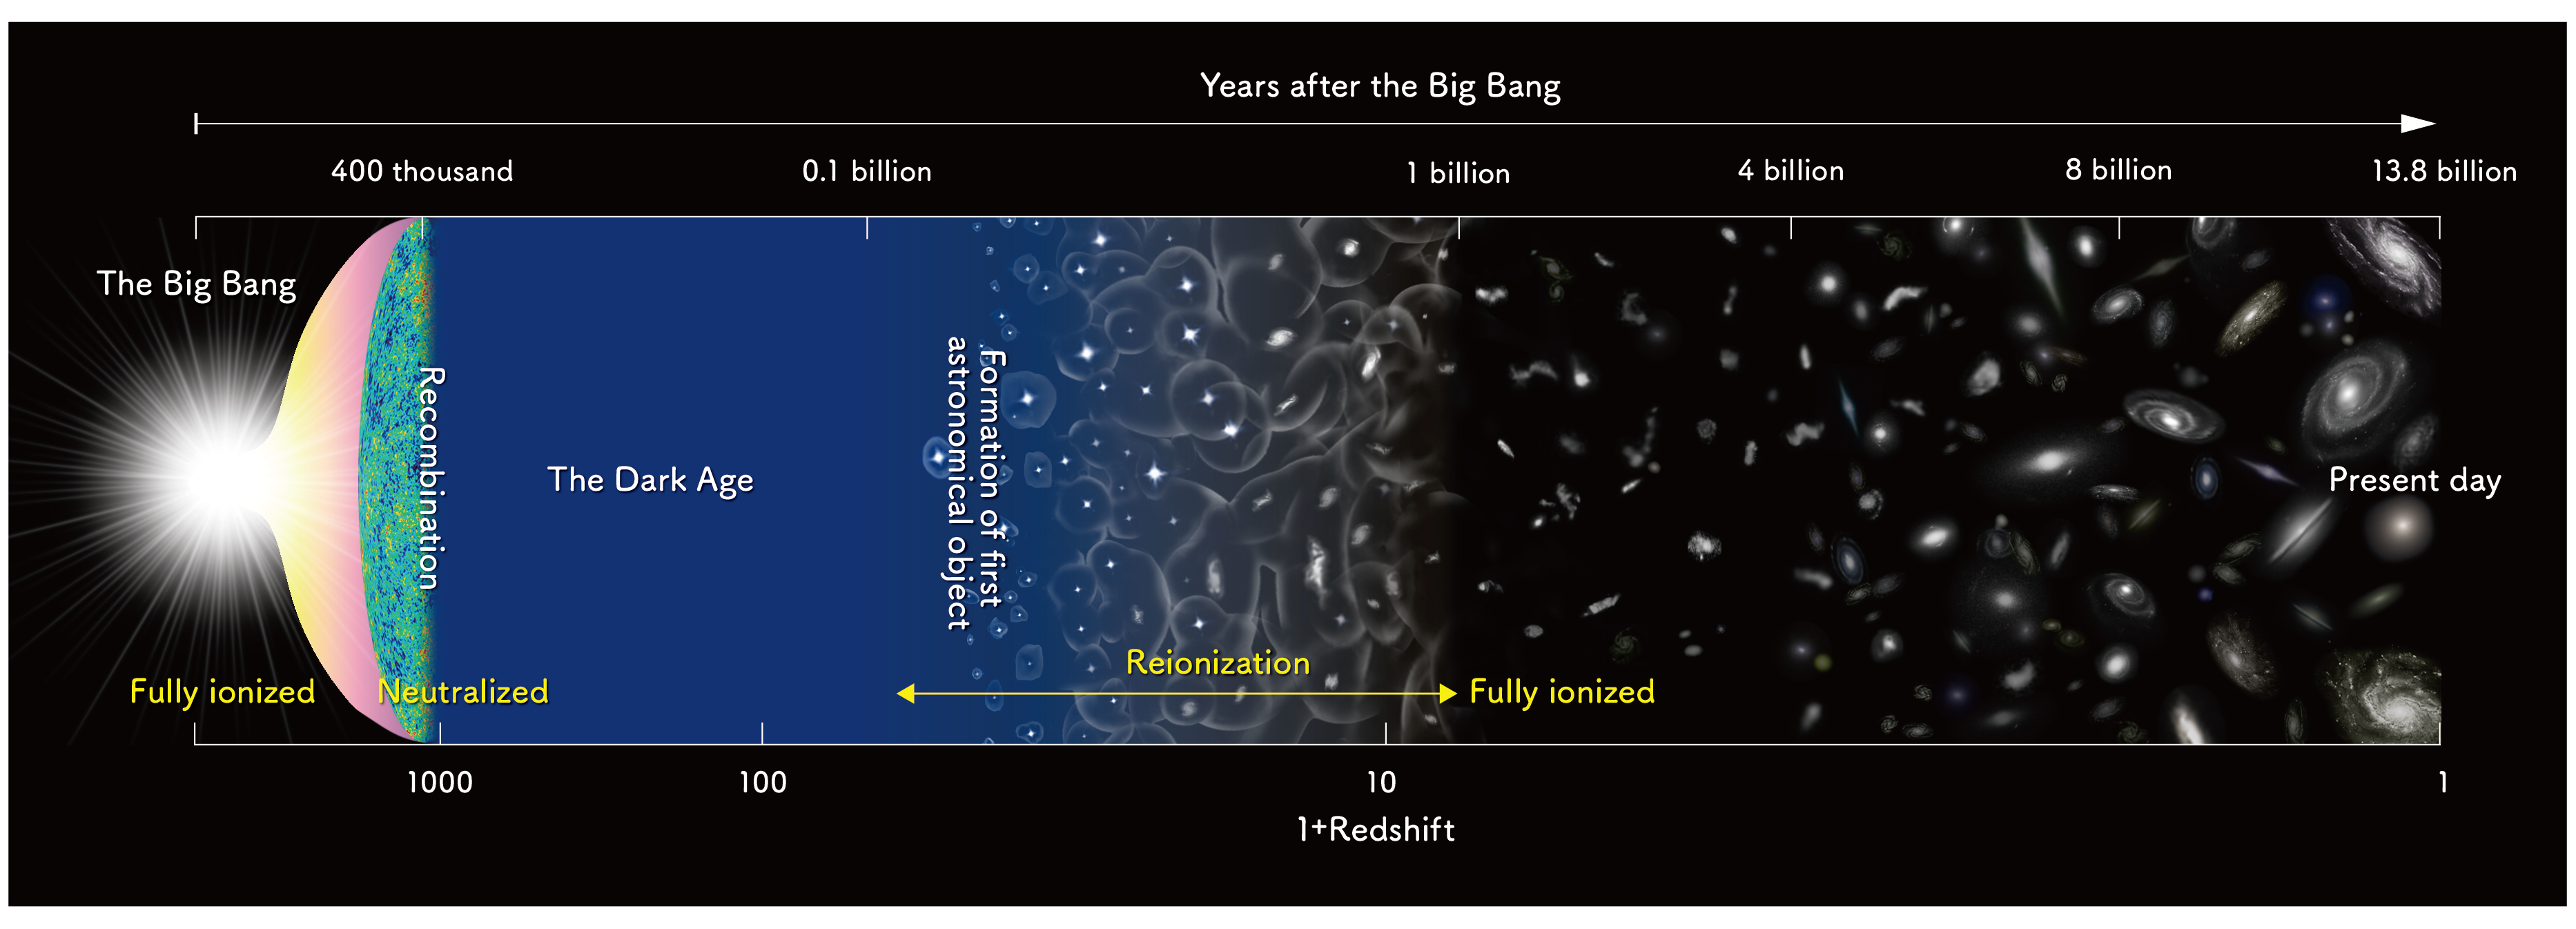
\includegraphics[width=\linewidth]{Figures/Reionizationtimeline.jpg}
			\caption{Cosmic history of the Universe.\protect\footnote{https://earthsky.org/space/cosmic-dark-ages-lyman-alpha-galaxies-lager}}
			\label{Fig:timeline}
		\end{center}
	\end{figure}
	
	Recombination (z $\sim1100$) occurred when the neutral hydrogen (HI) was formed from the cool enough Universe. Before that, electrons were not bound to protons, and the Universe contained ionized plasma known as photon-baryon fluid. Decoupled photons then formed the CMB. The first instance of the CMB was observed by~\citep{1965ApJ...142..419P} after the Era of Recombination. The telescopes that braced the Big Bang theory were the Cosmic Background Explorer (COBE)~\citep{2004astro.ph..2528M}, Wilkinson Microwave Anisotropy Probe (WMAP)~\citep{2009ApJS..180..306D}, Planck~\citep{2016A&A...594A..16P} and several subsequent ground-based telescopes~\citep{2004astro.ph..2528M}. Subsequently, the HI became the dominant baryonic component of the intergalactic medium (IGM). This was before the first stars' formation during the Dark Ages (z $\sim1100$ - z $\sim30$). There was rapid cooling of gas relative to the CMB. If the hydrogen can be mapped in this era, valuable cosmological data can be produced~\citep{2015Sci...349..849H, 11, 2004PhRvL..92u1301L}.\\
	
	There were density fluctuations in the distribution of matter, and the overdense regions collapsed under the influence of gravity, ultimately creating the first stars. Thus, nuclear reaction resulted into Cosmic Dawn (z $\sim30$ - z $\sim10$). An enormous emitted energy from the stars reionizes the Universe causing ionization. This further results in stars exploding due to gravitational disintegration leading to the formation of galaxies. There is a decelerating effect in the Universe expansion due to the force of gravity within dominating matter~\citep{2015Sci...349..849H, 2017arXiv170808521D, 2012AdSpR..49..433B}.\\
	
	Throughout the cosmological epochs, what is known is minimal because it is a challenge to observe them directly. Nevertheless, the contemporary occurrence of \SI{21}{cm} cosmology has imparted the capability of bridging the gap between what is known and what is not know about the eras of our history~\citep{2014ApJ...782L...9V, 2013PhRvD..87d3002L}.
	%such wealth of the Universe's history observations were            
	
	\begin{equation}
	\delta{T_b}\propto {x_{HI}}(1+z)^{1/2}({T_s}-{T_{CMB}})/{T_s}
	\end{equation}
	
	\begin{figure}[htb!]
		\begin{center}
			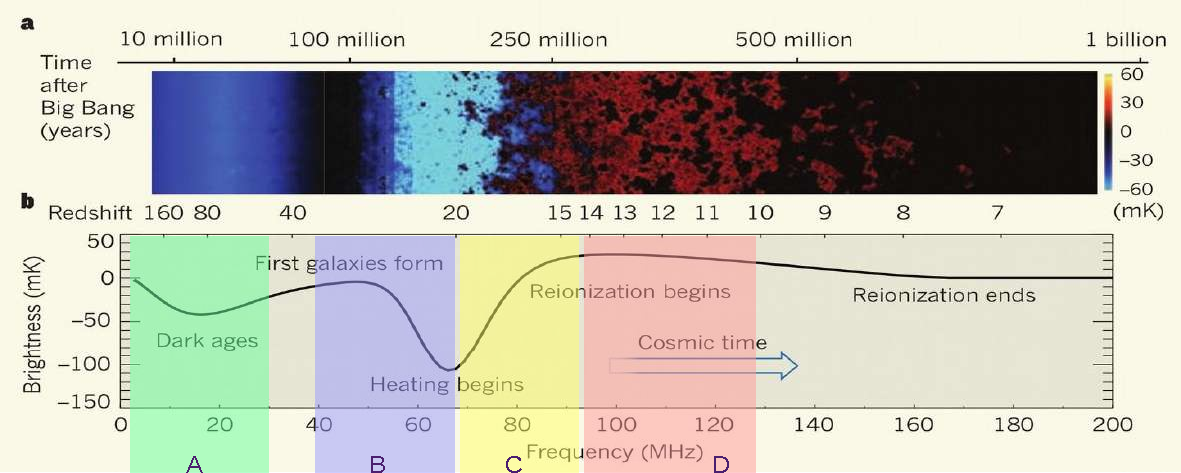
\includegraphics[width=\linewidth]{Figures/epo.pdf}\\
			\caption{Frequency structure of the globally averaged 21 cm signal~\citep{2012RPPh...75h6901P}} 
			\label{Fig:epochs}
		\end{center}
	\end{figure}
	
	
%	The brightness temperature ($\delta$$T_b$) that is measured depends on different important factors which are \(x_{HI}\), the fraction of neutral hydrogen, redshift ($z$) and two temperatures, the spin temperature ($T_s$) and the CMB temperature ($T_{CMB}$). 

%There is a difference in that the brightness temperature tend to be positive. Starting on the early times, the two important temperatures are the spin temparature and kinetic temperature of the gas. The differences there, are that the spin tempature tells us about the population of the hydrogen that is in the higher energies in parallel state. 
%	%What is happening in the spin temperature in conjuction with the kinetic temperature
	\subsection{Dark Ages}
	
	The cosmic Dark Ages is an epoch that is in the middle of Recombination (z $\sim1100$)and the Epoch of Reionization (z $\sim30$) from $\sim 380,000$ years until about 1 billion years at T = $\sim3000$ K~\citep{2014arXiv1412.2096J} where there was no existence of luminous sources.  It possesses distinctive features that have never been explored to date. Three sources are used to couple the Hydrogen spin temperature ($T_S$) in the IGM during its history. These sources are namely the kinetic gas temperature where the thermal motion of atoms is characterized in the gas. The 21 cm brightness temperature relative to CMB ($\delta$$T_b$), which provides a source of external 21 cm radiation. And the external optical photons corresponding to transition energies between the ground and excited state of the Hydrogen atom~\citep{2015aska.confE...1K,2006PhR...433..181F}.\\
	
	Right after Recombination, the IGM was dense enough for Compton scattering between CMB photons and free electrons in the IGM to set $T_K$=$T_\gamma$=$T_S$. During this period, light and matter separated from the CMB at z $\sim200$ and was cooled adiabatically as the Universe expanded, which led to $T_K$ decreasing below $T_\gamma$~\citep{2006PhR...433..181F}. \autoref{Fig:DA} shows one model prediction for the relevant temperatures including $T_\gamma$, $T_K$, $T_S$ and $\delta$$T_b$ before star formation. The CMB flux must have been resonantly absorbed by the cosmic neutral hydrogen through its spin-flip 21 cm transition before the first stars formed. At this juncture, the most dominating matter in the Universe was the dark matter and meager amounts of ordinary matter (neutral hydrogen and helium). After a few hundred million years, the dark matter which was predominant started to collapse into halo-like structures through gravitational collapse steadily cumulating physical matter and finally forming the first stars and galaxies, and that was the end of the cosmic Dark Ages~\citep{2003Sci...300.1904M}.

	\begin{figure}[htb!]
		\begin{center}
			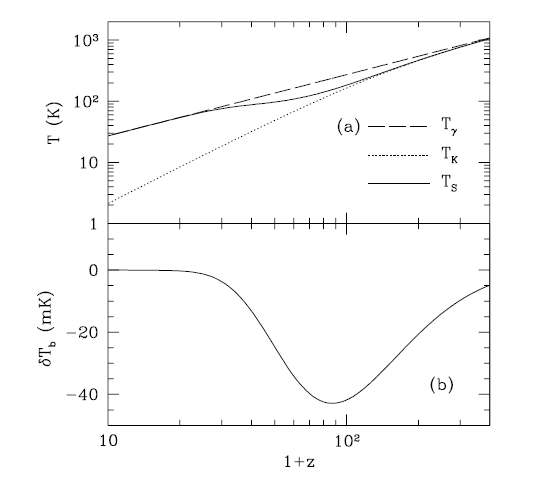
\includegraphics[width=0.7\linewidth]{Figures/DA.png}\\
			\caption{(a) Plot of $T_S$, $T_\gamma$, and $T_K$ during the Dark Ages, as calculated from initial conditions given by the CMB and (b) $\delta$$T_b$ during the same period with only collisional coupling present. Plots taken from~\citep{2006PhR...433..181F}} 
			\label{Fig:DA}
		\end{center}
	\end{figure}
%	
%\textcolor{red}{These stars, called Population III (since heavier elements were not produced in the big bang) are hypothesized to consist of only hydrogen and helium and thought to form in dark matter minihalos at a redshift of $z \sim20$ with masses 1-100 million times that of the sun~\citep{2016RvMP...88a5004C, 2007ApJ...660..516T}. These haloes are much smaller than the ones that dominate the universe today, as the universe was so young that today’s typical galaxies had not yet had time to form. Even small amounts of metals allow cooling of gas, necessary to form stars with masses similar to that of the sun. Thus, Population III stars are expected to be extremely massive ($\sim$ 100 solar mass) and highly luminous objects that ionised their neutral hydrogen surrounding, radically altering the properties of the Inter-Galactic Medium (IGM), imparting a characteristic structure in the brightness temperature of the globally averaged 21 cm sky signal as a function of frequency~\citep{2014ApJ...782L...9V}.\\}
%
%
%\textcolor{red}{The formation of this frequency structure is a result of the emission of Lyman Alpha photons by the first stars, strongly coupling the kinetic and spin temperatures of the IGM via the WouthuysenField effect (WF). At the birth of the first stars, the WF sets the kinetic and spin temperatures equal, lending to a drastic absorption signal in the mean brightness temperature of the IGM at the frequency of the first stars turning on. Later on, X-ray emission from the first generation of galaxies heats the IGM leading to a 21 cm emission signal, setting the beginning of reionisation~\citep{2014ApJ...782L...9V}. Hence, the global 21-cm signal captures the heating processes of the IGM by the first stars and is expected to have a 100 mK dip around 70 MHz, as shown in Figure 1. This signature is undetected to date, and a number of international experiments are working to make the first measurement ofthe universe in this slice of its history~\citep{2017ApJ...835...49M}.}	
%	
	\subsection{Cosmic Dawn}
	    
	    After the first stars' formation, their UV radiation couples to the HI line through the Wouthuysen-Field effect. The significant absorption HI feature is created by this coupling, which can be used to probe the first stars' spectra, with the potential of differentiating between Pop II and Pop III stars. The X-rays are emitted by hot accretion disks around the first stellar remnants (e.g., black holes), that effectively heat the cold HI gas (The gas surrounding these stars was both radiated and heated. By the Wouthuysen-Field (W-F) effect, the cold gas temperature was coupled from the spin-temperature. The second period (the Cosmic Dawn) originated where the hydrogen line was seen in absorption. As the stars continued to form, it is believed that there was an appearance of the first X-ray emitting sources, heating the neutral gas and thereby (again via the W-F effect) raising the overall spin-temperature to higher than the CMB temperature.\\
	    
	    
	    Consequently, the 21-cm line became visible in emission at $z\sim15$. During radiation and heating, these first sources (possibly including mini-quasars) also ionized the gas around them, and a period of Reionization started that is thought to have lasted until $z\sim5~to\sim 6$~\citep{2015aska.confE...1K}). During this period, the HI feature observations are sensitive to the black hole's properties and the progenitor's metallicity, offering further insight into first-star formation.~\citep{11}.\\ 
	    
	    By $z\sim 30$, collisions had become so rare that $T_S$$\approx$$T_\gamma$ , and the 21 cm fluctuations are no longer visible. However, at just about this time, the first collapsed objects began to form. These, and the surrounding networks of sheets and filaments, produced hot, overdense gas where collisional coupling became efficient again. Thus the next phase in the 21 cm history is the birth of the first nonlinear structures;~\citep{2006PhR...433..181F}. For that reason, observing the redshifted 21 cm emission of neutral hydrogen will educate us about what is unknown to date about the Universe's early phases and open a new observational window~\citep{2015aska.confE...1K}.  
	    
	\section{Cosmology with Redshifted 21-cm Emission}
	
%	\textcolor{red}{High redshift observations of the globally averaged 21-cm emission of neutral hydrogen has been recently proposed as a window into the cosmic dawn, an epoch of cosmic evolution that occured roughly a few hundred million years after the big bang, when the first stars ignited in the universe~\citep{2012RPPh...75h6901P}.\\}
	
	
	Observations of redshifted 21 cm line of neutral hydrogen at radio frequencies are a rapidly growing area of cosmology research that can potentially shed light on numerous epochs in the Universe's history.

	Our Universe is rich in the hydrogen gas, hence a
	concerted effort in the experimental community to develop telescopes for mapping neutral hydrogen via \SI{21}{cm} emission wavelength line. The \SI{21}{cm} wavelength of hydrogen gas is being observed by several experiments that are modeled for Hydrogen mapping in our Universe. This hydrogen line is an essential mechanism as it helps in the probing of the dark ages to the epoch of reionization (EoR)~\citep{2013PhRvD..87d3002L,2014ApJ...782...66P}.
	
	The generation of the hydrogen line (\SI{21}{cm} line or HI line) is due to the intrinsic spin of the hydrogen atoms, namely, an electron and the proton~\citep{book:832129}.\\
	
	The electron and proton spins can be oriented in either the opposing or the same direction respective to each other. When they are in an opposing direction, they result in an antiparallel spin, which implies that the hydrogen atom is in the lower energy state. When they are in the same direction, they result in a parallel spin, which implies that the hydrogen atom is in the higher energy state. Once an electron transition from one state to another, the hydrogen atom discharges a photon with a \SI{21}{cm} wavelength equivalent to (\SI{1420}{MHz}). The hyperfine splitting of the two energy states equivalent to \(\Delta E =  5.9 \times 10^{-6} \ eV\) is a consequence of the dissimilarity between the spin states.
		
	\autoref{Fig:21cm}\footnote{https://www.skatelescope.org/radio-astronomy/} shows the spin-flip transition process~\citep{16, book:832129}.
	
	\begin{figure}[htb!]
		\begin{center}
			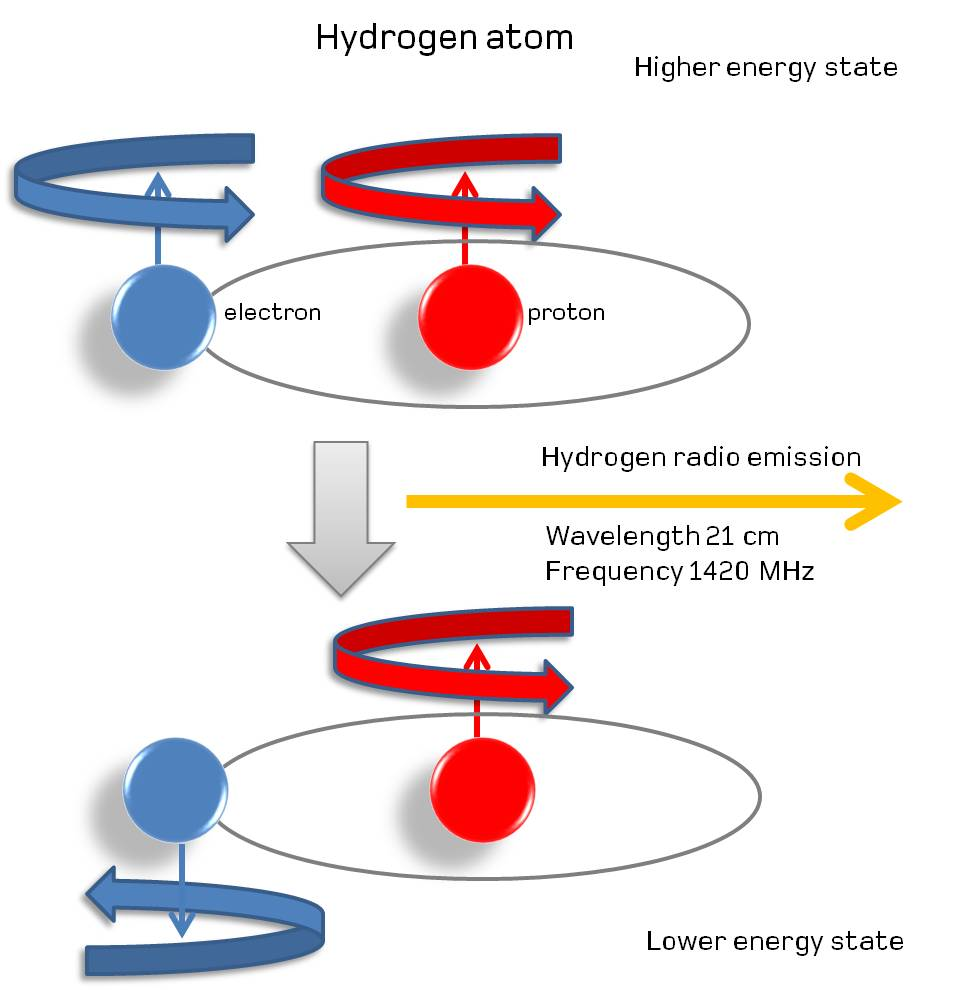
\includegraphics[width=0.5\linewidth]{Figures/Hydrogenemission1.jpeg}
			\caption{The formation of the \SI{21}{cm} wavelength line by the process of spin flip transition where the hydrogen atom moves from one energy state to another.}
			\label{Fig:21cm}
		\end{center}
	\end{figure}
	
%	The \SI{21}{cm} hydrogen line is redshifted as it moves further away. It is redshifted as far as z $\sim1000$, which corresponds to the cosmological dark ages and which puts the emission at low frequencies ranging from \SI{1.4}{MHz} to \SI{140}{MHz}. This is mathematically represented by the relationship between wavelength and redshift which is given by
%	\begin{equation} \label{eq1.1}
%	\begin{split}
%	1+z & = \frac{\lambda_{obs}}{\lambda_{emit}}= \frac{1}{a}
%	\end{split}
%	\end{equation}
%	where $z$ is the redshift, $\lambda_{obs}$ is the wavelength of the observed signal, $\lambda_{emit}$ is the wavelength of the emitted signal, and $a$ is the Universe expansion scale factor.
	
	\subsection{Hydrogen Line Observational Challenges}
	
	Since our Universe is rich in hydrogen, and the long-wavelength radiation can penetrate dust, this \SI{21}{cm} radiation is an ideal tool for probing the history of the Universe at any epoch of interest. However, the ground-based telescopes and experiments are faced with a challenge when it comes to using the \SI{21}{cm} highly redshifted line emission to observe the dark ages, cosmic dawn, and the Epoch of Reionization~\citep{2016ExA....41..271R}. The challenges are namely human-made Radio Frequency Interference (RFI), foregrounds, ionospheric interferences, and the instrumental systematics, which is non-transparent below \SI{10}{MHz}. 
	
	\subsection*{Brightness of Foreground Emission}
	
	The	primary challenge is the extreme brightness of foreground emission, contributed by both Galactic and extragalactic sources.
	The brightness temperatures of the foreground emission are 4-5 orders of magnitude brighter than the brighness temperature of the cosmological \SI{21}{cm} signal which is $\sim$ 0.14 mK at $z\sim0.8$~\citep{2018RAA....18..114H}.
	
	The Galactic synchrotron emission is primarily included in the foregrounds at low frequency, which originated from the cosmic ray electrons' movement in the Galactic magnetic field. Free electrons scattering off ions without being captured produces the Galactic free-free emission. The extra-galactic foregrounds are predominanntly radio-loud galaxies and quasars~\citep{2018RAA....18..114H, 2008MNRAS.389.1319J}.

	\subsection*{Instrumental Systematics}
	
	There needs to be a precise calibration of instrumental systematics to remove instrument effects from the data.
		
	Instrumental systematics further complicate this effort, causing foreground signal to contaminate Fourier modes in the data that would otherwise only be noise limited. Instrumental systematics have limited many of the current upper limits on the 21 cm power spectrum. Therefore, precise modeling and separation of instrumental systematics will likely be necessary for second-generation 21 cm observations to make sturdy observations of the 21 cm cosmological signal. Instrumental systematics includes calibration errors, ionospheric faraday rotation, primary beam ellipticity, analog signal chain imperfections (such as impedance mismatches), internal instrument couplings, such as signal chain reflections and antenna cross-coupling (i.e., crosstalk)~\citep{2020ApJ...888...70K}.
	
	
	
	\subsection*{RFI}
	
	Besides astrophysical challenges, human-made RFI saturates the frequency bands, increasing the need for isolated remote deployment sites. 
	
	The brightness of the RFI on the 21 cm observations can have up to orders of magnitude beyond the Galactic and extra-galactic foregrounds. Unfortunately, RFI introduces a reduction in sensitivity in two separate but distinct ways, one being the direct contamination by having similar spectral characteristics and overpowering of the 21cm signal. The other is the introduction of a complex sampling function due to missing data. This produces correlations between modes when computing the Fourier transform along the frequency axis (Offringa et al. 2019). Therefore,  identifying RFI while not falsely identifying non-RFI as RFI is crucial, further complicating our sampling function over frequency~\citep{2019MNRAS.488.2605K}.
		
	\subsection*{Ionospheric Contamination}
	
	The Earth's ionosphere also introduces significant fluctuations, which becomes increasingly refractive and turbulent below 100 MHz and becomes practically opaque below 10 MHz. Also, "filled aperture" antennas (typically paraboloidal reflectors), commonly used as interferometer elements at higher frequencies, become impractically large below 100 MHz; therefore, beamforming arrays consisting of many low-gain elements must be used instead. Examples of such arrays include the 22-MHz narrowband dipole array at Penticton, British Columbia, active during the 1960s~\citep{2005ITAP...53.2480E}.\\
	
	
	In order to minimize RFI and ionospheric contamination, there have been proposals to observe long wavelengths from space-based telescopes further away from the ionosphere of our planet. These space-based telescopes do not exist yet, and there are several ground-based experimental efforts to understand how well we can make measurements from Earth~\citep{2016ExA....41..271R}. \\
	
	
%	\textcolor{blue}{ This section should give a high level overview of what 21-cm measurements can tell us about the universe, across all redshifts.  In case it's helpful, I'll point you to a review talk that I gave about 21-cm measurements last year: (and we can chat about it on Wednesday if you'd like).  This section should also discuss global vs fluctuation measurements. }

	\section{Previous Cosmic Dawn and Low-frequency Experiments}
	
%	\textcolor{blue}{One subsection can be devoted to global signal experiments for cosmic dawn, and the other subsection can discuss <30 MHz imaging.  Keep in mind that your goal here isn't to recite the details of all experiments to date (so on that note, you don't need a separate sub-subsection for each experiment), but to describe the landscape and to set the context for your work.  Think about the unifying, big-picture aspects.  For example, for the global signal cosmic dawn experiments, focus on the primary design drivers: small antennas to measure total power, spectrally smooth behavior, RFI-quiet spots, etc.  You don't need to describe exactly how each instrument is built; you just want to give the reader a general sense of what these instruments broadly look like, how many there are, and where they exist.}
	
	
	Even with the challenges that are encountered in doing the 21 cm cosmology, several experiments nevertheless use the \SI{21}{cm} Hydrogen line to study the evolution of the Universe. These experiments are aimed at observing different epochs of the Universe including Dark Ages (z $\sim1100$ - z $\sim30$), cosmic dawn (z $\sim30$ - z $\sim10$) and Epoch of Reionization (z $\sim10$ - z $\sim2.5$). \\
	
%	\textcolor{red}{EDGES, SARAS2, LEDA, CTP, Bighorns, etc}
		
		\subsection{Global Signal Experiments for Cosmic Dawn}
		
		EDGES, BIGHORNS, LEDA
		
		\subsection{Imaging below 30 MHz}
	
	
%	The Long Wavelength Array (LWA) experiment operating at a frequency range of \SI{10}{MHz} to \SI{88}{MHz} is in correspondence with the redshift of $15<\text{z}<142$ and is aimed at probing the cosmic dawn and the dark ages \cite{2010iska.meetE..24H}. EDGES \cite{2018AAS...23111604M} has the same aim. The PRIZM \cite{2018arXiv180609531P} experiment probes the cosmic dawn only. The frequency and redshift ranges are shown in \autoref{table:range}. OVRO-LWA \cite{2018AJ....156...32E} probes EoR to cosmic dawn. GMRT-EoR \cite{2013MNRAS.433..639P}, PAPER \cite{2010AJ....139.1468P},MWA \cite{2009IEEEP..97.1497L} and HERA \cite{2017PASP..129d5001D} probes EoR. LOFAR \cite{2013A&A...556A...2V} probes from the Era of Acceleration to the Dark Ages. The frequency and redshift ranges are shown in \autoref{table:range1}. \\			
%	
%	
%	\begin{table}[h!]
%		\centering
%		\begin{tabular}{|c | c | c | c| c|} 
%			\hline
%			& EDGES &  PRIZM & LWA \\ [0.5ex] 
%			\hline
%			Frequency Range (MHz) & 50 - 190 & 70 - 100 & 10 - 88\\
%			\hline
%			Redshift Range & $\approx$ 28 - 6.5 & $\approx$ 19 - 13 & $\approx$ 142 - 15 \\
%			\hline
%		\end{tabular}
%		\caption{EDGES, PRIZM and LWA frequency and redshift ranges}
%		\label{table:range}
%	\end{table}
%	
%	\begin{table}[h!]
%		\centering
%		\begin{tabular}{|c | c | c | c | c | c |} 
%			\hline
%			& GMRT-EoR &  PAPER & MWA & HERA & LOFAR\\ [0.5ex] 
%			\hline
%			Frequency Range (MHz) & 150 & 139 - 174 & 70 - 300 & 50 - 250 & 10 - 240\\
%			\hline
%			Redshift Range & $\sim$ 8.5 & $\sim$ 9 - 7 & $\sim$ 19 - 4 & $\sim$ 6 - 30 & $\sim$ 142 - 5 \\
%			\hline
%		\end{tabular}
%		\caption{GMRT-EoR, PAPER, MWA, HERA and LOFAR frequency and redshift ranges}
%		\label{table:range1}
%	\end{table}
		{\bf{Long Wavelength Astronomy}}
	   
	    
	    The father of radio astronomy, Karl G. Jansky, played a massive role in the inauguration of radio astronomy dating back to 1931. At that time, he was an employee at the Bell Telephone Laboratories as a radio engineer. Jansky was allocated to study and solve the problem that hindered the radio communication systems. Using highly directive antenna arrays shown in \autoref{Fig:Jansky}, he discovered that the radio frequency noise that hindered the communication systems was caused by the static from thunderstorms~\citep{book:BasicsofRA, book:RA}.\\
	    
	    \begin{figure}[htb]
	    	\begin{center}
	    		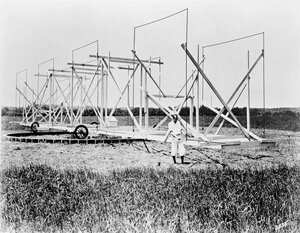
\includegraphics[width=\linewidth]{Figures/jansky1.jpg}
	    		\caption{Jansky's highly directive antenna arrays which he used to discover the cause of RFI that hindered the communication systems at Bell Telephone Laboratories~\citep{book:BasicsofRA}}.
	    		\label{Fig:Jansky}
	    	\end{center}
	    \end{figure}
	    The antenna that he constructed operated at an approximated frequency of \SI{20}{MHz}, corresponding to an approximate long wavelength of \SI{15}{m}. He further found radio radiation from the Galactic Center at the operating frequency. Out of interest in Jansky's instigating discoveries, Grote Reber designed a radio telescope that operated at a range of approximately \SI{10}{MHz} to \SI{160}{MHz} (\SI{30}{m}-\SI{2}{m} wavelength) in 1937. He discovered that the authoritative source at longer wavelengths was the Milky Way area. Furthermore, he realized that the radio telescope acts like a bolometer, or a device to measure the heat. The radiation resistance of the antenna measures an equivalent temperature of a distant part of space to which the 24 antenna response pattern projects it~\citep{1988JRASC..82...93R, CosmicStatic,2012PASP..124.1090H}.\\[0.1cm]
	    
	    Because of the research done for the communication systems, radio astronomy was born and expanded to fields of radio astronomy and astrophysics~\citep{2012PASP..124.1090H}. This led to an accelerated discovery of the hydrogen line research area, which was allocated an operating frequency of \SI{1420}{MHz} (\SI{21}{cm} wavelength)~\citep{10.2307/530765}. After all these discoveries, the long-wavelength astronomy fascination has been resuscitated in the present epoch.
	    
	    {\bf{Long Wavelength Astronomy Experiments}}
	    
%	    In the past, tens of years ago, there have been funds allocated to the long-wavelength experiments that exist and which are yet to exist. There are quite a few low-frequency experiments, but this document will briefly discuss LWA (\autoref{Fig:LWA}\footnote{https://phys.org/news/2011-01-astronomer-field.html}) based in the Very Large Array (VLA site). Further discussion will be on the few measurements that exist at $\lessapprox$ 30 MHz. Two of these experiments represent the lowest frequencies measured to date (Reber's antenna, RAE-B). The other two represent the highest resolutions achieved in this frequency range (DRAO, OVRO-LWA).\\
%	    
%	    {\bf LWA:} It is based in New Mexico on the Very Large Array (VLA) site. Its operating frequency ranges between \SI{10}{MHz} - \SI{88}{MHz} (wavelength between \SI{30}{m}- \SI{3.41}{m}) and is made up of incorporated beams which are from digitized 258 dual polarisation dipoles. The functionality of the first station of this project was finalized in 2011. The LWA possess distinctive multiskilled abilities to measure cosmic evolution, astrophysical plasma, relativistic particles, decametric radio radiation from Jupiter - like extrasolar planets and giant flares from magnetars. The final LWA is aimed at consisting of 53 phased array stations, which are steered electronically with as far as \SI{400}{km} baseline~\citep{2012JAI.....150004T,2010iska.meetE..24H}. \\
%	    
%	    
%	    \begin{figure}[h!]
%	    	\begin{center}
%	    		\includegraphics[width=0.5\linewidth]{Figures/LWA.jpg}
%	    		\caption{Several LWA Telescopes in New Mexico (VLA site)}
%	    		\label{Fig:LWA}
%	    	\end{center}
%	    \end{figure}
%	    
%	    \begin{figure}[htb]
%	    	\begin{center}
%	    		\includegraphics[width=0.7\linewidth]{Figures/LWA256.jpg}
%	    		\caption{All 256 LWA Telescopes in New Mexico (VLA site)~\citep{2012PASP..124.1090H}}
%	    		\label{Fig:LWA256}
%	    	\end{center}
%	    \end{figure}
%	    
%	    Comprehensive reviews of experimental efforts exist elsewhere, but none have made measurements at the lowest frequencies of $\lessapprox$ 30 MHz. This is due to the challenges, namely, the ionosphere, RFI, Galactic emission, and instrumental systematics~\citep{2018arXiv180609531P}. \\ 
	    
	    \textcolor{red}{Grote Reber came up with state of the art by constructing a telescope operating at very low frequencies between 0.52 MHz and 2.1 MHz, which had 192 dipoles. At 2.1 MHz, it had a resolution of as low as $\sim$5 \degree. This experiment at 2.1 MHz created the keymap of the sky. He also mentioned that his measurements were influenced by galactic emission and the ionosphere~\citep{article, 1988A&A...195..372W}. The Radio Astronomy Explorer-2 (RAE-2) has significantly low operating frequency ranges between 25 kHz - 13 MHz, it main science goal was to do radio astronomy evaluation of our Galaxy (the Milkyway), the Sun, Eart and all the other planets. The resolution of this experiment is $\sim$10 \degree at 4.7 MHz~\citep{1975A&A....40..365A}. Both of these experiments made very low-resolution measurements.\\}
	    	
	    \textcolor{red}{The experiments which made the high-resolution measurements are the OVRO-LWA 36 MHz experiment, Dominion Radio Astrophysical Observatory (DRAO) 22 MHz telescope, and the DRAO Penticton 10 MHz array. The OVRO-LWA operates at frequency ranges of 36.528 MHz and 73.152 MHz. At these frequencies, it has an angular resolution of \SI{15}{\arcminute}~\citep{2018AJ....156...32E}. The DRAO telescope operated at 22 MHz, and its resolution ranges between $\sim$1.1 \degree - 1.7 \degree. Its primary science goal was to measure the emission from discrete sources and observe our Galaxy's emission from its environment~\citep{1999A&AS..137....7R}. The DRAO 10 MHz array operated had a resolution of $\sim$ 2  \degree, and it was first used for discrete sources and was later used to map the large-scale structure of the background radiation~\citep{1976MNRAS.177..601C}.}
	    
	\section{Structure of this Thesis}


\chapter{Marion Island Site}

        \section{}
\chapter{\prizm~Instrumentation}
    \section{\prizm~Experiment Overview}
    \section{Signal Chain}
        \subsection{}
        \subsection{}
        \subsection{}
    \section{Revised \prizm~Instrumentation}
        \subsection{}
        %With your permission, may I please include the \prizm\ new front end here  
        \subsection{}
	
\chapter{\albatros~Experiment}

%Array of Long Baseline Antennas for Taking Radio Observations from the Sub-antarctic
    \section{Overview of the Pathfinder}
    \section{Pathfinder System Signal Chain}
	    \begin{figure}
	    	\begin{center} 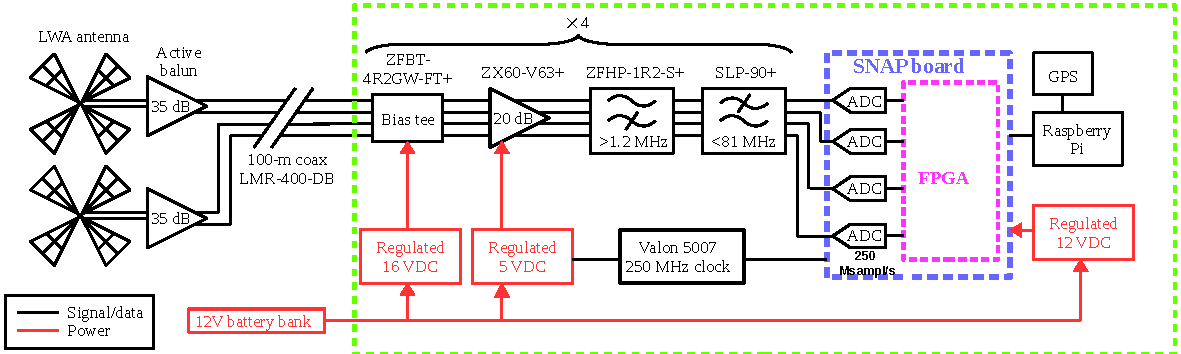
\includegraphics[width=\linewidth]{Figures/pathfinder_schematic.pdf}
	    		\caption{Two-element \albatros\ pathfinder block diagram.  Signals
	    			from two dual-polarzation LWA antennas are amplified by
	    			front-end active baluns~\citep{2012PASP..124.1090H}.  The
	    			antennas are connected via 100-m coaxial cables to the back-end readout electronics, which are housed in a Faraday cage denoted by the dashed box.  Each of the four antenna outputs is passed to a second-stage electronics chain consisting of filters and	further amplfication.  The signals are digitized at 250~Msamp/s by a SNAP board, which includes an on-board FPGA that computes
	    			auto- and cross-spectra from and between the four inputs.  A Raspberry Pi controls the SNAP board and saves the data.}
	    		\label{Fig:albatros2_schem}
	    	\end{center}
	    \end{figure}
   
        \subsection{}
        \subsection{}
        \subsection{}
        \subsection{}
        
        
\newpage
    \section{Overview of Autonomous Stations}
    \section{Autonomous Stations Signal Chain}
    
    \begin{figure}
    	\begin{center}
    		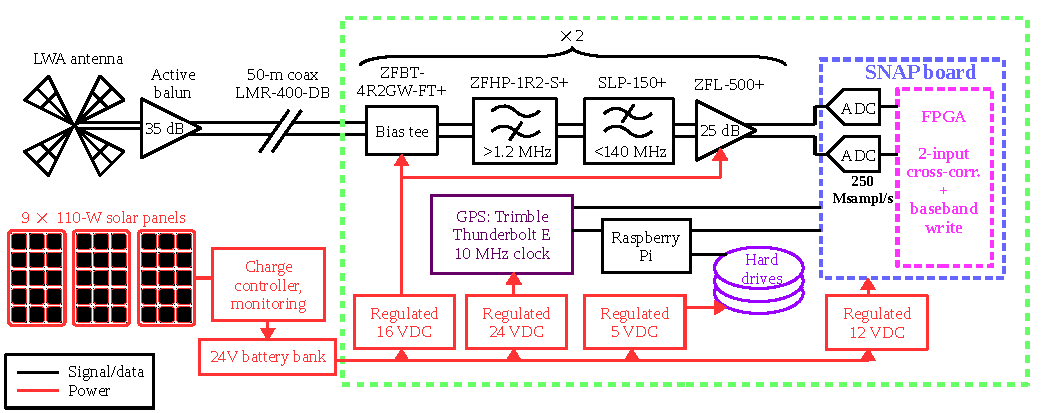
\includegraphics[width=\linewidth]{Figures/albatros_single_schematic.pdf}
    		\caption{Single-antenna autonomous station block diagram.  A dual-polarization LWA antenna, equipped with a front-end active balun, connects via 50-m coaxial cables to the back-end readout electronics, housed in a Faraday cage denoted by the dashed box. Each of the two antenna signals is passed to a second-stage	electronics chain consisting of filters and further amplfication.  The signals are digitized at 250~Msamp/s by a SNAP board, which includes an on-board FPGA that computes channelized baseband and spectra from both inputs.  A Raspberry Pi controls the SNAP board and receives the baseband data and spectra.  The baseband data are saved to external hard drives. The system is powered by solar panels that charge a 24-V battery	bank.}
    		\label{Fig:albatros1_schem}
    	\end{center}
    \end{figure}
    
        \subsection{}
        \subsection{}

\chapter{Preliminary Data and Recommendations}

\bibliographystyle{unsrtnat}                                                         
\bibliography{TH_Moso_MSc_Thesis}{}
    

\end{document}
